\section{Introduction}
%RENAN - 1 pag

Hydropower has an important share in the global electricity production, and
will continue to be a major source of renewable
power-generation\footnote{International Energy Agency (2010), http://www.iea.org/.}% \cite{iea}.
. In hydropower generating plants, the average maintenance cost is 2\% of the
investment cost per kW, and, typically, the large mechanical
components, as turbines, must be maintained and replaced every 25 years.
The cavitation and abrasion phenomena on the turbine's blades have become a
concern, as the erosion can lead to water flow instability, excessive
vibrations and turbine efficiency reduction \cite{goldemberg2007energia}. Hard
coating techniques by thermal aspersion are used to greatly increase the life
cycle of runner's blades~\cite{krella2011new}.

In the specific case of Brazil, hydropower is the largest
power-generation source. To support future economic growth, Brazil has
invested in additional large hydroelectric facilities, for instance, the
14~GW Belo Monte along the Xingu River\footnote{Energy
Information Administration (2014), https://www.eia.gov/.}%~\cite{eia}
, and Jirau dam (Fig.~\ref{fig::jirau_turb}) along the Madeira river. At the
latter, the high concentration of suspended particles carried by the river intensifies the abrasion phenomena, thus
regular maintenance is needed. Currently, blade coating maintenance in these
large facilities is performed before turbine assembling by a large-sized
robotic manipulator. 

Repair maintenance, as grinding and welding, can be done manually in the
turbine's environment, but the hard coating procedure requires a robotic system
due to high precision, speed, and the usage of hazardous substances.
There are several difficulties encountered when attempting to robotize
\textit{in situ} maintenance, as accessibility, system placement and
calibration. A few robotic systems have been investigated to perform \textit{in
situ} repair of turbine runners, as it could greatly improve efficiency and
safety, but none has been used for the hard coating operation. Some examples found in the literature are:

\begin{figure}[h!]
\centering
	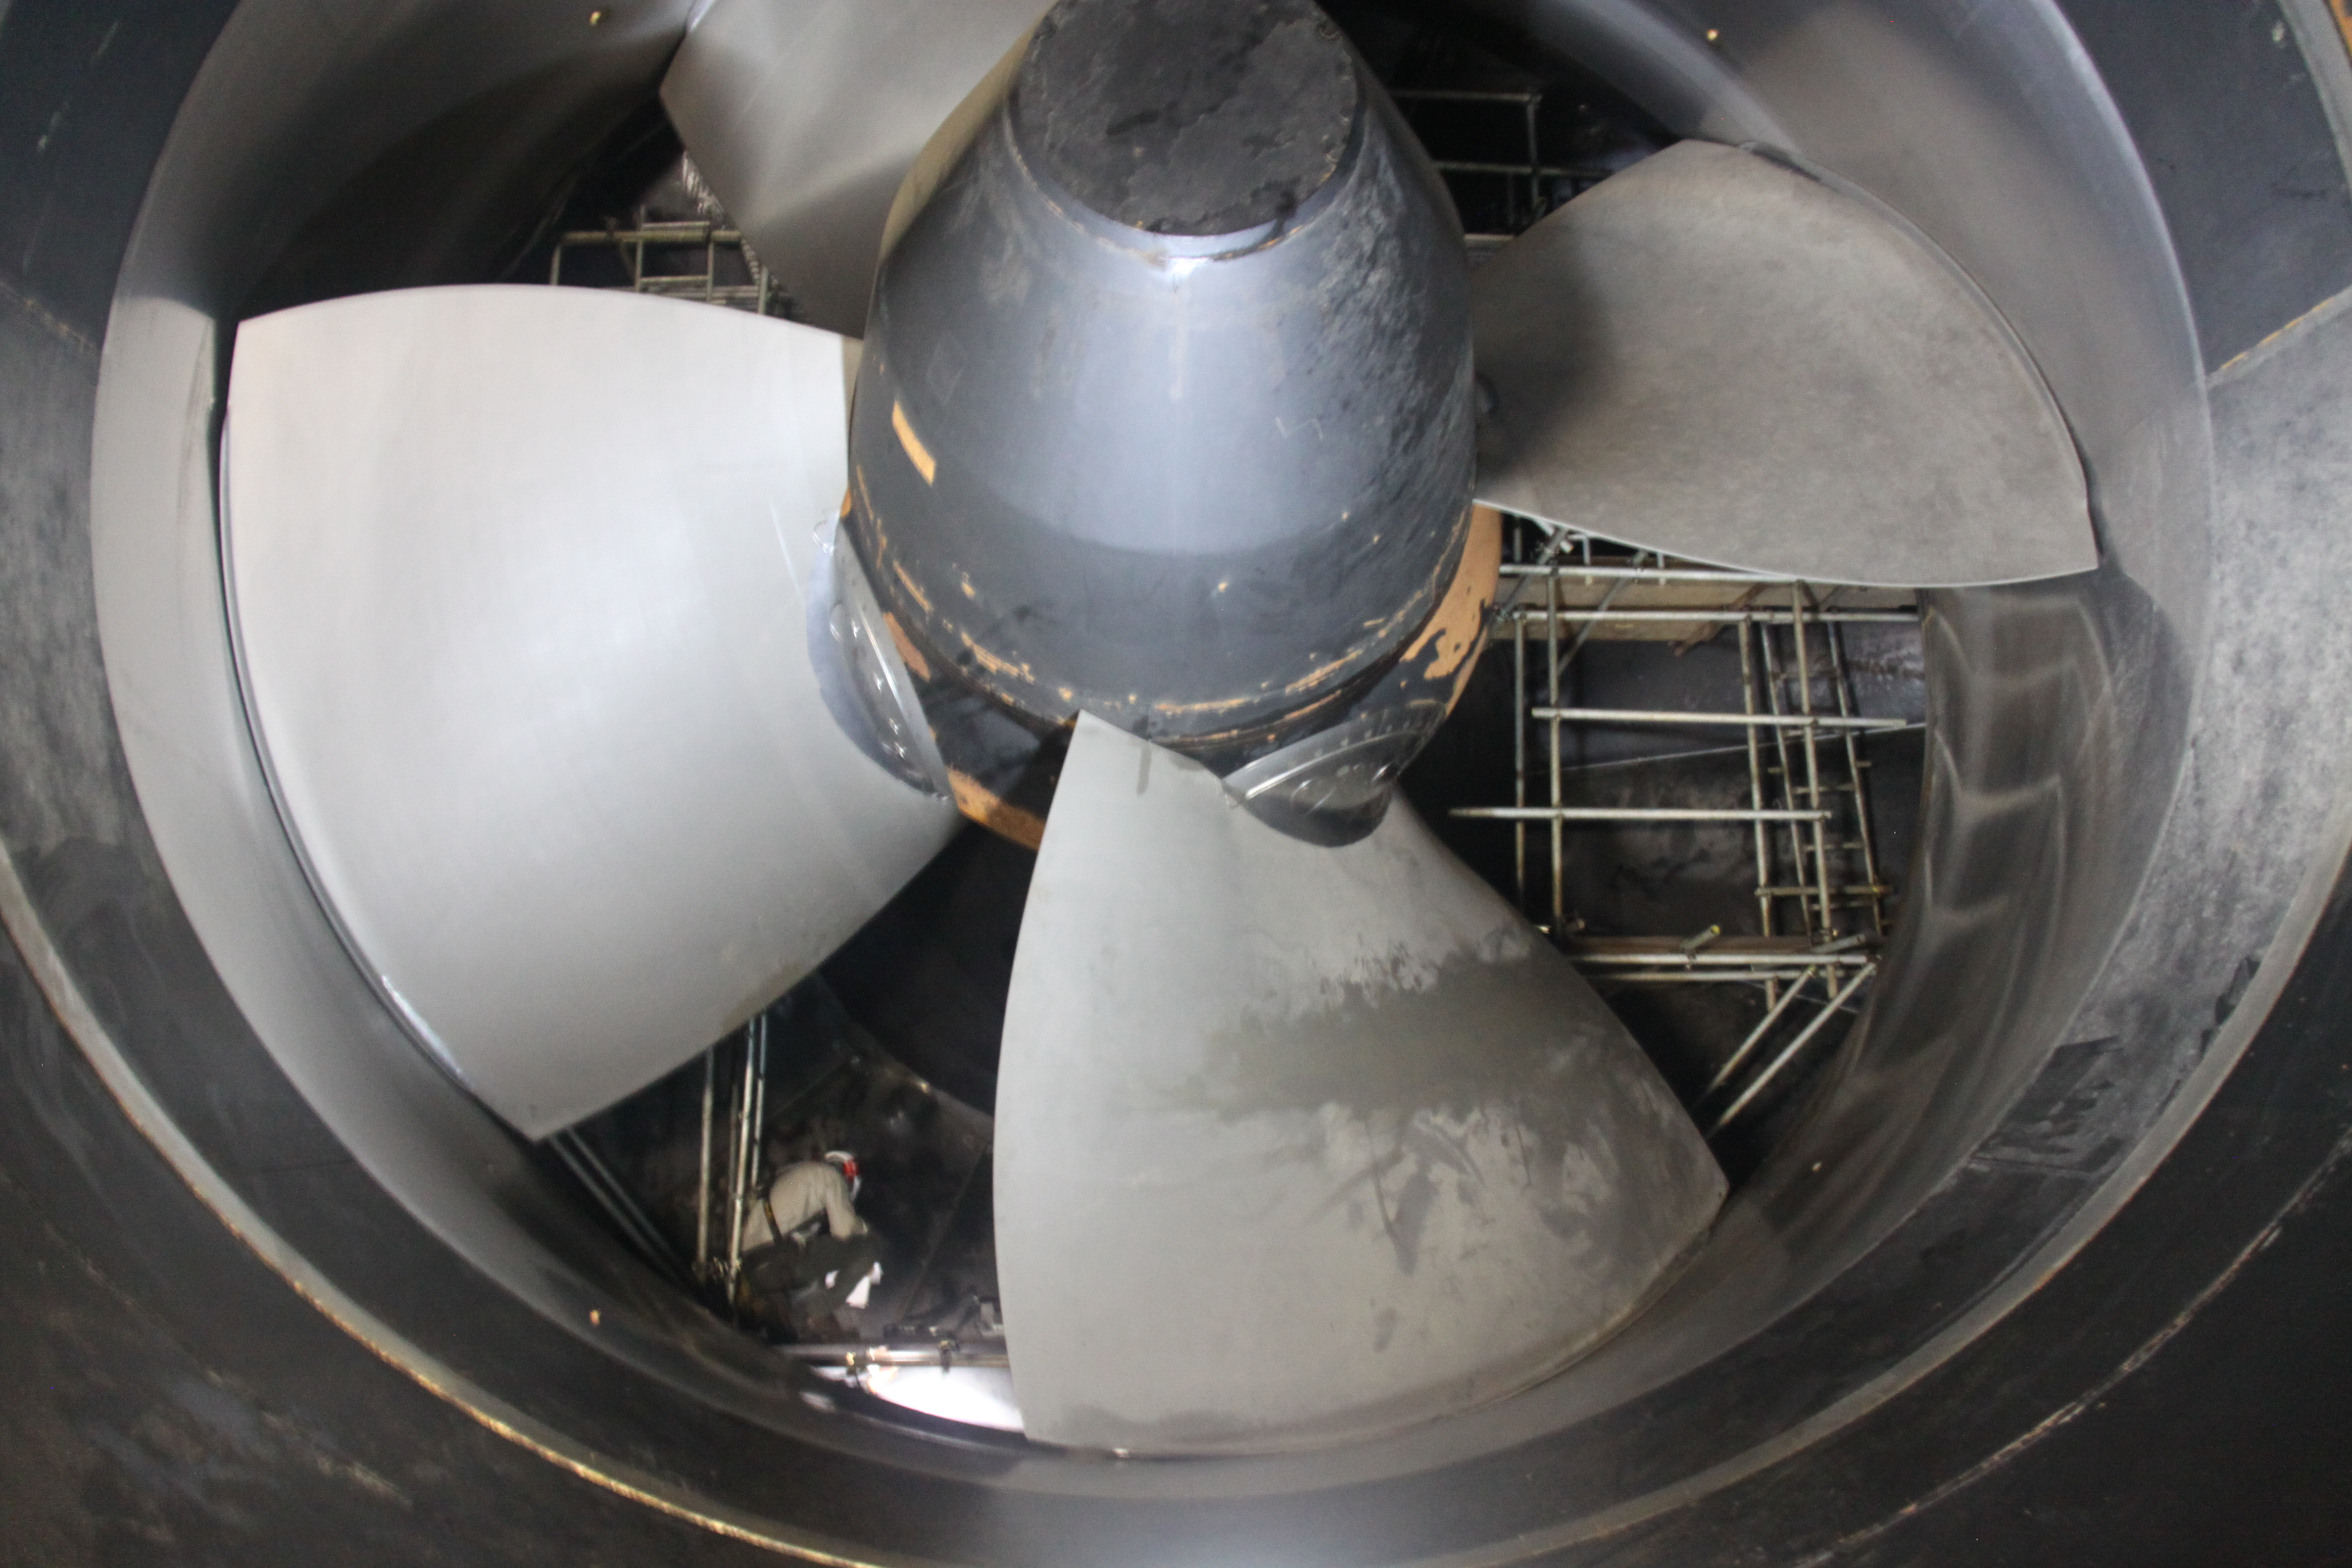
\includegraphics[width=.8\columnwidth]{figs/intro/jirau_turb.JPG} 
	\caption{Jirau's hydropower turbine.}
	\label{fig::jirau_turb}
\end{figure}

\begin{itemize}
\item The Roboturb~\cite{roboturb} and the Scompi~\cite{scompi} are robotic
systems to perform erosion inspection and welding on damaged runner's blades.
They move on a flexible rail, which may be shaped and then fixed to the blade
surface.

\item \textit{The Climber}\footnote{International Climbing Machines (2013),
http://www.icm.cc/.} %~\cite{icm}
 is an intervention robot for wind and hydroelectric turbines, to perform
coating removal, surface cleaning and coating application. It is a climbing
robot with pneumatic adhesion and locomotion by tracks.
\end{itemize}

In this paper, we present a general overview of a robotic system called EMMA,
and a detailed description of the mechanics, the manipulator, and
calibration. The system performs \textit{in situ} hydropower
runner's blade hard coating.


\begin{comment}
, and it is composed of an industrial manipulator
that moves on customized rails, a 3D laser scanner for mapping, and
sensors for positioning feedback.
The system operate in a confined space, move
on a sloping and slippery environment through a rail, identify the runner's
blades, calibrate its position, generate the path planning and perform the hard
coating. 


This text is organized as follows: a general overview of the robot and its main
challenges are presented in Section \ref{sec:general_overview}, detailed
descriptions of the embedded electronics, the vehicle support system, power
supply system, and software architecture are taken in
Sections \ref{sec:electronics_overview}, \ref{sec:powersupply_overview}, and
\ref{sec:software} respectively.
In Section \ref{sec:results}, preliminary results are shown, and concluding
remarks are drawn in Section \ref{sec:conclusions}.
\end{comment}